\section{Como fizemos?}

O objetivo central desta pesquisa é abrir a caixa-preta do discurso naturalizado de que ``qualquer um pode editar'', e verificar como ele se constrói e se sustenta na materialidade cotidiana da Wikipédia. Utilizamos o termo caixa-preta conforme definido por Bruno Latour (\citeyear[p. 4]{latour_ciencia_1987}), como algo sobre o qual ``\textit{não é preciso saber nada, a não ser o que nela entra e o que dela sai}''. Assim, para abrir esta caixa-preta, não nos bastará apenas olhar para as funcionalidades colaborativas do software e para os grandiosos números de produção de conteúdo. Como Latour, que ao estudar a construção de fatos e artefatos, diz que ``\textit{nossa entrada no mundo da ciência e da tecnologia será pela porta de trás, a da ciência em construção, e não pela entrada mais grandiosa da ciência acabada}'' (\citeyear[p. 6]{latour_ciencia_1987}), analogamente fizemos a mesma entrada com a Wikipédia, nos ocupando de estudar não seus verbetes prontos, mas o funcionamento cotidiano de suas engrenagens de produção desses verbetes. Assim, não estudamos ``\textit{as coisas 'em si', mas as coisas 'entre si'. Mais importante que as coisas 'nelas mesmas', são suas relações, suas associações}'' \cite[p. 13]{feitosa_cidadao_2010}.

O conceito de caixa-preta, como definido por Latour, é um dos elementos centrais dos Estudos de Ciências-Tecnologias-Sociedades (CTS) que suportam esta pesquisa. Originado na cibernética para se referir a sistemas que seriam muito complexos para serem detalhados, o conceito é empregado como uma representação de uma entidade que recebe uma entrada e fornece uma saída, devendo-se assumir que funciona perfeitamente para seu propósito, sendo desnecessário preocupar-se com seu funcionamento. Latour então utiliza este termo para falar de verdades científicas e artefatos tecnológicos que se naturalizam e são aceitos a priori, sem controvérsias. Assim, abrir uma caixa-preta, seria o movimento de entender como os fatos e artefatos foram construídos (\citep[p.31]{latour_ciencia_1987}). É exatamente neste sentido que utilizaremos o termo ao longo da pesquisa.

A tentativa de entender o funcionamento da enciclopédia com o ferramental metodológico dos Estudos CTS, eleito como balizador desta pesquisa, levou a não observá-la como algo estanque, mas como um organismo vivo, em fluxo. Assim, para entender as dinâmicas da comunidade wikipedista, o presente trabalho foi conduzido com duas abordagens complementares: ``de dentro para fora'' e ``de fora para dentro''. A primeira configurada pelos processos de tomada de decisão e naturalização de regras na Wikipédia em português, e a segunda pela chegada de editores/as novatos/as e as barreiras enfrentadas por eles/as.

Em ambas as abordagens de pesquisa anunciadas utilizamos ferramentais tanto de pesquisas qualitativas como quantitativas, acompanhando densamente trilhas de discussões, históricos de decisões e alterações em ferramentas automatizadas com o olhar próximo e míope de uma formiga – trocadilho usado por Latour, dado que a sigla em inglês para Actor-Network Theory (ANT) tem o mesmo nome do inseto -, ao mesmo tempo em que nos ocupamos de observar quantitativamente suas repercussões e implicações em todo o ecossistema da enciclopédia, com o olhar abrangente e amplo de uma águia.

Dando sequência a apresentação do arcabouço metodológico da pesquisa, é lançada mão da Teoria Ator-Rede (TAR), utilizada para tratar dos enredamentos e estabilizações de fatos científicos e artefatos tecnológicos. Sabemos que fatos e artefatos têm sua própria dinâmica de construção (\cite{fleck_genesis_2010}), mas o caso de artigos na Wikipédia se aproxima bastante dessa dinâmica, e os estudos sobre a construção de textos científicos caem como uma luva para estudos de escritas enciclopédicas. Como diz Esteves (\citeyear[p.102]{esteves_as_2014}), “\textit{a Teoria Ator-Rede propôs definir a factualidade de uma alegação não em termos de uma suposta veracidade intrínseca, mas nos termos de sua resistência aos ataques que ela venha a sofrer. A analogia com a Wikipédia é clara. Latour parecia descrever a verificabilidade nessa passagem de Ciência em ação: ‘E a que resiste [a realidade]? Aos testes de força. Se, numa dada situação, nenhum dissidente for capaz de modificar a forma de um novo objeto, então é isso, é realidade, ao menos enquanto os testes de força não forem modificados’ (\citep[p.93]{latour_ciencia_1987})}”. Neste caso, ou seja, uma vez que cessaram provisoriamente as controvérsias, os/as especialistas e os laboratórios não estão imersos nas controvérsias pela escrita da realidade, mas os/as editores/as da enciclopédia assumem o papel de seus porta-vozes e a disputa, apesar de deslocada, segue dinâmicas similares.

Assim como o fazer da ciência, a escrita da Wikipédia também segue um “\textit{caminho muito estranho porque é invisível quando tudo vai bem}” (\citep[p.44]{latour_cogitamus_2010}). Porém, quando existem divergências entre editores/as, suas redes de aliados que sustentam verbetes instáveis tornam-se visíveis, e publicações científicas, relatórios da ONU, notícias de jornais e demais fontes são arregimentadas por wikipedistas para defender uma versão do texto do verbete. A busca por aliados/as mais poderosos/as para reforçar uma posição dá a impressão de se assemelhar ao que ocorre na tecnociência a tal ponto que a seguinte passagem de Latour (\citeyear[p.48]{latour_cogitamus_2010}), sobre a estrutura textual de publicações científicas poderia muito bem ter sido escrita sobre verbetes da Wikipédia: “\textit{a presença ou ausência de referências, citações e notas de rodapé é um sinal tão importante de que o documento é ou não sério que um fato pode ser transformado em ficção ou uma ficção em fato apenas com o acréscimo ou a subtração de referências”}.

Nos moldes de um “A vida da Wikipédia como ela é", esta pesquisa se apoiará sempre que possível em relatos de casos concretos do cotidiano da enciclopédia que demonstrem a não trivialidade de enquadramentos e fronteiras estanques, colocando uma lupa sobre situações de panes, transbordamentos e recomposições. Pois afinal, são nesses momentos em que as caixas-pretas tornam-se nada óbvias. O seu processo de estabilização (ou não), que permitirá a existência de momentos posteriores estáveis de funcionamento, é exatamente o ponto de interesse da pesquisa. Como ensina Feitosa (\citeyear[p.9]{feitosa_cidadao_2010}), "\textit{um fazer ou estudar tecnologia comprometido em evidenciar as decisões tecnopolíticas relevantes para certos coletivos, deve tentar entender e explicar a relação entre artefatos e esses coletivos, ou seja, deve tentar explicar como as coisas ditas técnicas e as demais entidades (humanas e não humanas) se relacionam, com o fim, inclusive, de indicar caminhos a serem seguidos ou evitados no fazer tecnologia}".


Se para todo enquadramento existe um transbordamento (\cite{callon_markets_1998}), é exatamente nas bordas onde se encontra nosso interesse de estudo. Na definição não trivial, maleável e instável de fronteiras, onde cotidianamente narrativas são configuradas e reconfiguradas no ecossistema da enciclopédia. Um exemplo prático que podemos brevemente citar, para ilustrar ao leitor o local de definição de fronteiras que nos interessa, é a controvérsia em torno da política editorial de verificabilidade da Wikipédia lusófona. Ela enuncia que ``\textit{pessoas lendo e editando a enciclopédia podem checar se a informação provém de uma fonte confiável. A Wikipédia não publica pesquisa inédita; todo seu conteúdo é determinado pela informação previamente publicada ao invés de se basear apenas nas opiniões, crenças e experiências de seus editores. Mesmo se você tem certeza de que algo é verdadeiro, isto deve ser verificável através das fontes da informação antes de você adicioná-lo}'' (\citewiki{ptwiki_verificabilidade}).

Mesmo que aparentemente formulada de forma ``clara'' e ``direta'', esta regra tem suas fronteiras de aplicação constantemente movimentadas por seus/suas usuários/as, que disputam incessantemente contornos entre noções de conformidade, bom senso, respeito e qualidade.

No contexto desta disputa foi criado, em 2011, o ensaio ``\textit{Você não precisa citar que o céu é azul}''. Dissertando sobre a política de verificabilidade, afirma que ``\textit{muitos editores não entendem corretamente a política de citação, e veem nela um mecanismo para obrigar, consolidar ou deixar dúvidas sobre um ponto de vista em particular em uma disputa, ao invés de usá-la apenas para validar a informação da Wikipédia. Isto acaba gerando diversas formas de comportamentos desestabilizadores que devem ser evitados}'' (\citewiki{ptwiki_nao_precisa_citar_ceu_azul}).

Logo após criado, o ensaio viu sua página de discussão ser palco de um acalorado debate, com mais de 46 mensagens feitas por 17 diferentes usuários/as, variando de discordâncias enfáticas a apoios ao ensaio ser tornado uma política oficial. As discordâncias ganharam robustez com a publicação de outro ensaio, em 2013, intitulado ``\textit{É preciso citar que o céu é azul}''. Neste novo ensaio, defende-se que ``\textit{alguns editores podem disputar factos\footnote{Os textos da Wikipédia lusófona podem ser escritos em qualquer das diversas versões do português. Optamos por manter a grafia original das passagens transcluídas e não as adaptar para o português brasileiro.} aparentemente simples e óbvios. Até mesmo a afirmação de que ‘o céu é azul’ pode ser questionada porque o céu muito frequentemente tem cores diferentes, e todas as informações prováveis de vir a ser disputadas precisam de fontes}'' (\citewiki{ptwiki_e_preciso_citar_ceu_azul}). O ensaio ainda acrescenta que o verbete ``\textit{Céu}'', desde 2008, apresenta como legenda de sua figura principal o seguinte texto: ``\textit{quando visto de uma certa altitude, como de um avião, o céu varia de cor}'' (\citewiki{ptwiki_ceu_definicao}).

\begin{figure}[H]
    \centering
    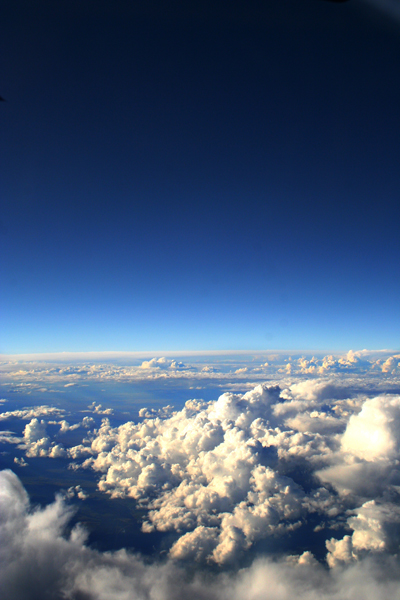
\includegraphics[width=0.4\textwidth]{Images/ceu.png}
    \caption{Imagem que ilustra o verbete “Céu” desde 2008.}
    \label{fig:ceu}
\end{figure}

Seguindo esta linha argumentativa, o ensaio conclui com as seguintes palavras: “\textit{Só porque uma coisa a si lhe parece óbvia, não significa que seja óbvia para toda a gente. Construa artigos unicamente a partir de fontes fiáveis de autoridades no assunto e cite essas fontes}” (\citewiki{ptwiki_e_preciso_citar_ceu_azul}).

Ambos os ensaios estão marcados com a predefinição ``Ensaio contestado'', que anuncia em uma caixa no topo das páginas de ambos ensaios: ``\textit{\textbf{Atenção}: Esta página contém um ensaio da Wikipédia que é seguido por parte dos seus editores, \textbf{mas é contestado por outro grupo de editores}}''\footnote{Grifos do original.} (\citewiki{ptwiki_predifinicoes_ensaios_contestado}). Ou seja, mesmo o primeiro ensaio tendo sido criado em 2011 e o segundo em 2013, até hoje, em 2020, nenhum deles foi reconhecido como uma política oficial da Wikipédia em português, e ambos contam com correligionários/as que convivem na enciclopédia com práticas antagônicas de aplicação da política de verificabilidade.

\begin{figure}[H]
    \centering
    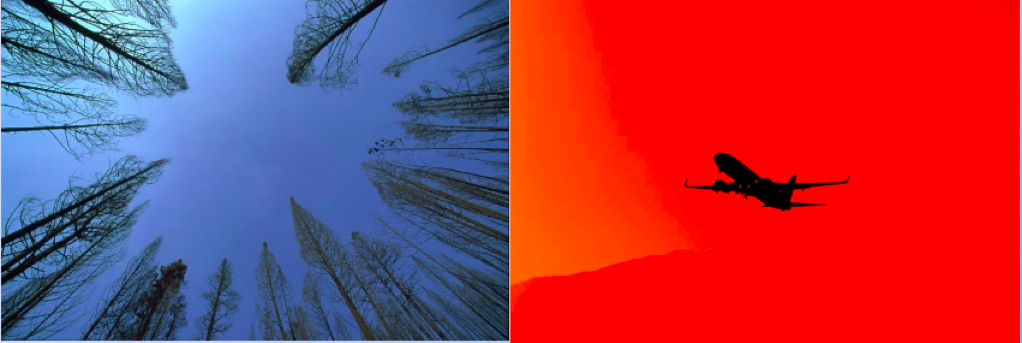
\includegraphics[width=1\textwidth]{Images/ceus-verificabilidade.png}
    \caption{Imagens que ilustram os ensaios que debatem as fronteiras de aplicação da política de verificabilidade.}
    \label{fig:ceus-verificabilidade}
\end{figure}

Situações como a relatada levaram nossa pesquisa a se interessar tanto pelos enredamentos que configuram a governança cotidiana da enciclopédia como pela forma que orientações nada triviais, como a demonstrada, podem se tornar barreiras no caminho de novos usuários que não tenha a experiência requerida para realizar devidos desvios para poderem editar.

A forma como a ambivalência de nossa pesquisa aqui citada se desenvolvera e fora implementada é então detalhada na seção a seguir.

% 
\subsection{Estudos quantitativos e a Wikipédia}

Metodologias quantitativas podem entrar em rota de colisão com os Estudos CTS, pois tendem a realizar inferências que confiam em metadados como fiéis porta-vozes dos fenômenos estudados, assim como tendem a dedicar pouca atenção às traduções\footnote{Utilizamos o termo ``tradução'' da mesma forma que  Bruno Latour, apoiados no conceito criado por Michel Serres em ``\textit{La traduction}'', de 1974, e retrabalhado em ``\textit{Le tiers-instruit}'', de 1991.}, traições, enquadramentos e transbordamentos que estão necessariamente envolvidos no processo de criação de camadas de conhecimento. Como proposto por Henrique Cukierman, em palestra no evento ``Avaliação da produção científica brasileira: pensando com a história das ciências'', organizado em 2011 pela SBHC e pelo HCTE\footnote{Sociedade Brasileira de História da Ciência (SBHC) e Programa de Pós-Graduação em História das Ciências e das Técnicas e Epistemologia da Universidade Federal do Rio de Janeiro (HCTE).}, sobre a confiança nos números, geralmente traduzida como ``objetividade'': ``\textit{O que há de especial com a linguagem da quantidade? Respondendo de forma sucinta, pode-se dizer que a quantificação é uma tecnologia de controle a distância, pouco ou nada relacionada com a chamada 'verdade' da natureza}'' (\cite[p.5]{cukierman_uma_2011}). Em seguida, citando Theodore M. Porter, ressaltou que ``\textit{a quantificação é parte de uma estratégia de intervenção, e não de mera descrição}'' (\cite[43]{porter_1996}, apud \cite[p.5]{cukierman_uma_2011}).

Na literatura de estudos sobre controvérsias na Wikipédia é comum encontrar pesquisadores/as caindo nesta armadilha da autoproclamada "objetividade" dos dados, realizando estudos profundos unicamente alicerçados em metadados que são assumidos como verdades puras e neutras, sem que os/as pesquisadores/as se ocupem em compreender como são elaborados, em observar quais ações foram de fato realizadas pelos/as usuário/as que viriam a gerar tais metadados estudados. É o caso sintetizado por Latour (\citeyear{latour_ciencia_1987}) como "\textit{o representante sendo assumido automaticamente como o representado}". 

Sigamos então com uma breve revisão bibliográfica para observar a materialidade desta prática de utilização dos metadados como porta vozes suficientes nos estudos mais citados sobre controvérsias na Wikipédia.

Em um trabalho bastante citado\footnote{89 citações segundo o Google Scholar. Página disponível em https://scholar.google.com.br/scholar?hl=pt-BR\&as\_sdt=0\%2C5\&q=Edit+wars+in+Wikipedia\&btnG= , acessada em 25 de março de 2020.}, “\textit{Edit wars in Wikipedia}”, Sumi et al (2011) propõem o índice M de controvérsia, observando “\textit{como' o número de edições e reversões desviam em algumas páginas dos números seguidos pela maioria dos artigos}”\footnote{Todas as citações desta revisão bibliográfica foram traduzidas livremente pelo autor.}. Mapeando duplas de editores/as que se revertem em um artigo e seu volume de edições no mesmo texto, os autores testam seu modelo em 6 diferentes idiomas e observam que menos de 1\% dos artigos apresentam um resultado significativo em seu índice.

O trabalho anterior foi a base do estudo ``\textit{The most controversial topics in Wikipedia: A multilingual and geographical analysis}'' de Yaseri e aliados, citado já 100 vezes por outros estudos.\footnote{https://scholar.google.com.br/scholar?hl=pt-BR\&as\_sdt=0\%2C5\&q=The+most+controversial+topics+in+Wikipedia\%3A+A+multilingual+and+geographical+analysis\&btnG= , acessada em 25 de março de 2020.} Nele foi utilizado o 
índice M como ponto de partida para observar versões em diferentes idiomas da enciclopédia buscando aproximações e similaridades entre grupos de idiomas próximos, com o objetivo explícito de criar ``\textit{um indicador multilíngue e independente da cultura}'' (\cite{yasseri_controversial_2014}). Em sua pesquisa, eles identificam que a maior parte das controvérsias são localizadas\footnote{Utilizamos ao longo desta pesquisa o termo ``localizada'' da mesma forma que o Movimento Wikimedia, adjetivando coisas que não sejam definidas globalmente pelo movimento, e podem ser instanciadas localmente de forma distinta pelas comunidades de cada projeto.}, e não se repetem tão comumente em outros idiomas (menos ainda se forem de grupos linguísticos diferentes), o que reforça a dificuldade de utilizar metadados globais para mapear comunidades com práticas distintas.

Já Vuong et al. (\citeyear{vuong_ranking_2008}), em “\textit{On ranking controversies in wikipedia: models and evaluation}”, com 115 citações\footnote{	https://scholar.google.com.br/scholar?hl=pt-BR\&as\_sdt=0\%2C5\&q=On+ranking+controversies+in+wikipedia\%3A\+models+and+evaluation\%E2\%80\%9D\&btnG= , acessada em 25 de março de 2020.}, resolvem levar em consideração não somente a atividade editorial em um artigo, como igualmente o perfil dos/as usuários/as envolvidos/as. Utilizando também a idade do artigo (em número de revisões salvas, e não em tempo corrido desde sua criação), os autores propõem diferentes índices partindo da seguinte premissa: “\textit{um/a usuário/a é mais controverso/a se participa de disputas em artigos menos controversos e um artigo é mais controverso se nele participam de disputas usuários/as menos controversos/as}”. Ambos os conceitos de controvérsia que se retroalimentam, tanto de usuários/as como de artigos, emergem de metadados brutos.

Em “\textit{There is no deadline: time evolution of Wikipedia discussions}”, o artigo menos citado desta revisão bibliográfica mas ainda assim com relevantes 32 menções\footnote{https://scholar.google.com.br/scholar?hl=pt-BR\&as\_sdt=0\%2C5\&q=There\+is+no+deadline\%3A+time+evolution+of+Wikipedia+discussions\&btnG= , acessada em 25 de março de 2020.}, Kaltenbrunner e Laniado (\citeyear{laniado_emotions_2012}) voltam-se para os metadados de edição das páginas de discussão dos artigos, onde inicialmente não encontraram padrões de volume de edições correlacionados com os metadados de suas páginas correspondentes no domínio principal. Aprofundando a inferência, criaram o indicador\textit{h}, que aponta o maior número de discussões que seja igual ao número mínimo de respostas nelas. Observando o tempo que um artigo leva para incrementar seu \textit{h}, o estudo procura “\textit{identificar escaladas ou estabilizações de controvérsias}” de forma totalmente automatizada.

Em “\textit{Visual analysis of controversy in user-generated encyclopedias}”, citado 97 vezes\footnote{	https://scholar.google.com.br/scholar?hl=pt-BR\&as\_sdt=0\%2C5\&q=Visual+analysis+of+controversy+in+user-generated+encyclopedias\&btnG= , acessada em 25 de março de 2020.}, Brandes e Lerner (\citeyear{brandes_visual_2008}) estão interessados em saber quem edita depois de quem, e qual a diferença de tempo entre essas edições. Com essas informações, o artigo cria uma visualização de usuários/as agrupados/as, simbolizando “facções” em disputas de edições. Neste caso, após gerar seus mapas a partir dos metadados, os pesquisadores buscaram ler os artigos e estudar o perfil dos/as usuários/as envolvidos/as nas disputas, tanto na versão inglesa da Wikipédia como na alemã. De forma não surpreendente para nós, após está análise qualitativa, concluíram que seu modelo tende a aproximar vândalos\footnote{Termo utilizado no Movimento Wikimedia para se referir a usuários/as que fazem edições de má fé.} e combatentes de vandalismo, pois “\textit{ambos podem apresentar o comportamento ‘um contra todos}’” (\cite{brandes_visual_2008}). Pensando em melhorias de seu trabalho que deem conta de fazer de forma automatizada tão importante distinção entre esses perfis de usuário/a tão claramente desiguais, propõem que sejam adicionados futuramente à equação mais metadados, tais como registros de bloqueios dos/as usuários/as e conversas realizadas nas páginas dos/as usuários/as.

Por fim, citamos o badalado\footnote{137 citações mapeadas no Google Scholar. Disponível em https://scholar.google.com.br/scholar?hl=pt-BR\&as\_sdt=0\%2C5\&q=Global+disease+monitoring+and+forecasting+with+Wikipedia\&btnG= , acessada em 25 de março de 2020.} trabalho “\textit{Global disease monitoring and forecasting with Wikipedia}”, de Generous et al (\citeyear{generous_global_2014}), que foi objeto de grande cobertura da mídia\footnote{Em uma rápida busca no Google ainda hoje é fácil recuperar matérias de veículos como Washington Post https://www.washingtonpost.com/news/to-your-health/wp/2014/11/13/how-wikipedia-reading-habits-can-successfully-predict-the-spread-of-disease/ , LA Times https://www.latimes.com/science/sciencenow/la-sci-sn-wikipedia-flu-disease-predictor-20141113-story.html e Revista Galileu https://revistagalileu.globo.com/Ciencia/Saude/noticia/2014/11/como-wikipedia-pode-ajudar-monitorar-doencas.html} ao buscar identificar, antes das autoridades de saúde pública, surtos de doenças epidêmicas a partir do comportamento dos/as usuários/as nas Wikipédias. Mesmo se esforçando em realizar calibragens locais, fica claro em seus resultados que enquanto muito bem-sucedidos (como alardeado pela imprensa) para algumas doenças em alguns países em um determinado recorte temporal, o modelo puramente baseado em metadados fracassou na maioria dos casos testados.

Como ficou claro, a tradição de utilizar ferramentas de ciência de dados e análise de metadados em pesquisas costuma caminhar em uma proposta metodológica antagônica à concepção CTS de abertura de caixas-pretas aqui defendida. O impasse apresentado em tentar simultaneamente acompanhar densamente dinâmicas locais e utilizar técnicas quantitativas generalizantes pode parecer então incompatível com os Estudos CTS.

Porém, nem tudo está perdido. Mesmo com alguma ressalva, Latour (\citeyear[p.167]{latour_cogitamus_2010}) relata em Cogitamus que “\textit{sim, reconheço, as ferramentas digitais são um veneno. Mas, talvez, também ofereçam um remédio. Ao menos, isso é o que exploro há dez anos com os alunos dos cursos chamados ‘mapeamento de controvérsias’. Talvez fosse possível aprender a se orientar nas disputas, com a condição de contar com uma plataforma suficientemente calibrada e padronizada, para dar a um público virtual – ainda a ser inventado – hábitos comuns}". Seguindo esta visão, podemos observar “\textit{As controvérsias da ciência na Wikipédia em português: o caso do aquecimento global}”, tese de doutorado defendida em 2014 por Bernardo Esteves. Em um grande esforço para estudar as controvérsias sobre mudanças climáticas utilizando ferramental metodológico CTS, Esteves (\citeyear[p.295]{esteves_as_2014}) observa que “\textit{na Wikipédia, cada ação dos editores deixa rastros disponíveis para consulta de pesquisadores e demais interessados, abrindo uma janela para um repositório riquíssimo de informações sobre como os usuários negociam suas versões de verdade}”, e, para dar conta desses rastros, acompanha editores/as, regras editoriais, robôs, bloqueios, discussões e proteções de páginas, narrando processos de resolução de controvérsias e de estabililização de textos enciclopédicos. Em sua pesquisa, Esteves fez tanto análises quantitativas como qualitativas, e em seus esforços de construir um olhar ao mesmo tempo amplo como o da águia e míope como o da formiga, chegou a cogitar a criação de um indicador de controvérsias que pudesse ser utilizado na Wikipédia em português imbricando estes olhares.\footnote{"\textit{Acreditamos que os resultados deste estudo poderiam ganhar mais refinamento e resolução caso tivéssemos explorado mais a fundo as ferramentas computacionais para extrair e tratar dados disponíveis na base de dados da Wikipédia. Ademais, os resultados de um tratamento estatístico mais robusto poderiam talvez contribuir para o desenvolvimento de um índice de controvérsia mais adequado às especificidades das interações ente os usuários da Wikipédia lusófona}" \cite[p.296]{esteves_as_2014}.}

Seguindo ainda outro exemplo da linha de “\textit{Mapping Controversies}” apresentada na citação acima de Latour, o Médialab do Instituto de Estudos Políticos de Paris (Science Po), o mesmo Instituto onde Bruno Latour trabalha, foi enredado com a Fundação Barcelona Media, ferramentas de visualização de dados, o DesityDesign Lab do Politécnico de Milano, metadados da Wikipédia, o Digital Methods Initiave da Universidade de Amsterdam e orçamentos de pesquisa da Comissão Europeia no Projeto Contropedia, em um esforço para “\textit{construir uma plataforma de visualização e análises em tempo real de controvérsias na Wikipédia”} (\cite{noauthor_site_2013})\footnote{Todas as citações de textos da Contropedia foram traduzidas livremente pelo autor.}. Criado em novembro de 2013, o projeto é brevemente mencionado por Esteves em sua tese, mas no momento de seu estudo praticamente não havia informações publicadas sobre o desenvolvimento do projeto. Agora, o projeto já tem resultados publicados e uma versão beta de sua plataforma disponível para uso, propondo-se a “\textit{prover um melhor entendimento de fenômenos sociotécnicos que acontecem na internet e equipar cidadãos com ferramentas para desenrolarem plenamente a complexidade de controvérsias}” \cite{noauthor_site_2013}.

Diferente dos demais estudos sobre controvérsias na Wikipédia  anteriormente citados, a Contropedia não se propões a medir quais artigos são controversos dentro de uma Wikipédia, e sim quais tópicos são controversos dentro de um determinado artigo. O índice de controvérsia da Contropedia é associado a \textit{wikilinks}\footnote{Link internos em verbetes da Wikipédia para outros verbetes dentro da enciclopédia.}, e é calculado somando edições com alguma remoção de conteúdo de frases onde o \textit{wikilink} apareça no artigo. Sendo que, caso mais de um wikilink apareça na mesma frase, o peso de controvérsia atribuído é proporcional ao número de wikilinks na frase editada \cite{borra_societal_2015}

Esse sutil deslocamento dos metadados utilizados se deve ao distanciamento do projeto dos esforços de criação de indicadores de controvérsia gerais, em direção a uma posição onde buscam apoiar quantitativamente pesquisadores/as que estejam observando detalhadamente a construção de artigos. A ferramenta se propõe então a ser um mapa que aponte indícios para pesquisadores/as que pretendam fazer investigações densas, chamando a atenção do/a pesquisador/a para tópicos dentro do artigo que ensejem um olhar mais aprofundado.

Concordamos com Erik Borra, que junto de outros pesquisadores do projeto Contropedia (\citeyear[p.196]{noauthor_site_2013}), afirma que ``\textit{reconhecer o potencial do histórico de edições da Wikipédia como provedor de insights sobre controvérsias sociais, e reconhecer que cada link em um artigo pode ser visto como um ponto focal de debate, nos permite utilizar a Wikipédia como um interessante local para mapear controvérsias}''. Esta afirmação ressona com as observações de Esteves (\citeyear[p.295]{esteves_as_2014}) segundo as quais ``\textit{até o fim do século XX, os cientistas sociais tinham que escolher entre análises quantitativas robustas que os distanciavam de seu tema de pesquisa ou análises qualitativas detalhadas que corriam o risco de perder de vista o contexto mais amplo em que seu objeto de estudo se inseria. [Os cientistas sociais] precisavam escolher entre falar muito sobre pouco ou pouco sobre muito. A difusão das ferramentas computacionais de análise de dados e a grande disponibilidade de registros deixados pelos usuários dos sistemas digitais na internet abriram novas possibilidades para as ciências sociais e tornaram viável superar ao menos em parte esse dilema}''.

É importante destacar na proposta de atuação da Contropedia a preocupação em ter a ferramenta como provocadora de insights, e não como uma instância julgadora que automaticamente decreta vereditos em nome do/a pesquisador/a. Como dito no próprio site do projeto, a ``\textit{Contropedia destaca conhecimento instável em oposição a fatos estáveis}'' (\cite{noauthor_site_2013}). Citando mais uma vez Latour, sobre a adaptação do uso de ferramentas quantitativas de ciência de dados para pesquisas CTS, “\textit{é como se houvéssemos passado da pesquisa dos matters of fact à exploração dos matters of concern”\footnote{Grifo do original.}} (\cite[p.160]{latour_cogitamus_2010}). Tomando esse ponto de vista, e tendo o devido cuidado de não buscar resolver as disputas estudadas mas orientar sua investigação, e atentando para o fato de que ``\textit{uma representação da realidade, quando transladada para um sistema de informação, é, inevitavelmente, representada em categorias sempre limitadas, previamente estabelecidas em estruturas de bancos de dados. [...] A maneira como essa classificação se dá, ou seja, a escolha das categorias para o enquadramento é uma questão importante, com efeitos para o coletivo}'' (\cite[p.8]{feitosa_cidadao_2010}), a aproximação que parecia improvável de ferramentas de análise quantitativa de dados com os Estudos CTS se torna possível.


\subsection{De dentro para fora e de fora para dentro}

A trajetória de nossa pesquisa começou em 2017, com o plano de dar sequência a um dos trabalhos futuros propostos pela tese de Bernardo Esteves\footnote{\textit{(...)os resultados deste trabalho também poderiam ser explorados com a cartografia de controvérsias, método de visualização das forças em oposição nas controvérsias proposto por pesquisadores alinhados com a Teoria Ator-Rede (\cite{venturini_diving_2010};\citeyear{venturini_building_2012}). As duas abordagens – um tratamento estatístico de maior escopo e a visualização com a cartografia de controvérsias – são duas perspectivas possíveis de desdobramento deste trabalho no futuro em parceria com outros pesquisadores.}" (\cite[p.296]{esteves_as_2014})} e investigar ferramentas de mapeamento e cartografia de controvérsias na Wikipédia. Em nosso esforço inaugural neste caminho foi produzido um primeiro artigo, ``\textit{Controvérsias na Wikipédia lusófona: pode o olhar CTS ser apoiado por ferramentas quantitativas?}'', apresentado no \textit{International Wikipedia Scientific Conference} (IWSC), que se propôs a ``\textit{revisar esforços prévios de mapeamentos de controvérsias na Wikipédia e analisar o funcionamento da ferramenta Contropedia, explicitando suas funcionalidades e a utilizando para observar algumas controvérsias, a fim de entender como ferramentas quantitativas podem apoiar estudos de controvérsias que utilizem abordagens CTS}'' (\cite[p.1]{de_andrade_controversias_2017}).

Após este primeiro resultado de nosso projeto de pesquisa, passamos a estudar \textit{in loco} diferentes práticas de escrita na Wikipédia, suas barreiras e resultados obtidos, com ênfase em possíveis peculiaridades da Wikipédia em português. 

Esta nova abordagem se materializou em uma apresentação feita no 6º Simpósio Nacional de Ciência, Tecnologia e Sociedade (ESOCITE.BR), intitulada “\textit{Histórias das ciências para todos: uma prática de escrita biográfica na Wikipédia em português}”, onde é “\textit{lançado um olhar CTS sobre a escrita de conteúdos enciclopédicos relacionados aos estudos de Ciências-Tecnologias-Sociedades, descrevendo três cenas de edição da Wikipédia acontecidas no contexto de uma disciplina de pós-graduação, cada qual com objetivos, enredamentos, desvios, alistamentos e resultados bem distintos}” (\cite{andrade_historias_2017}).

No desenvolvimento das duas abordagens de pesquisa abertas foi possível observar que o onipresente discurso de que “\textit{todos podem editar}” não se mostrava na prática tão óbvio como colocado pela comunidade, e o interesse por sua exploração passou então a figurar como tema central da investigação que segue. Este movimento se soma a leitura da dissertação “\textit{O discurso do global nas comunidades de software livre: estudo de caso do WordPress}”, defendida por Rodrigo Primo no Programa de Engenheria de Sistemas e Computação da COPPE/UFRJ, em 2017, na qual problematiza o discurso de adesão e representatividade global da comunidade que desenvolve o Wordpress, CMS\footnote{Do inglês Content management system, são sistemas de publicação e gerenciamento de páginas online.} mais utilizado do mundo. Sua problematização é construída a partir do estudo das dinâmicas de funcionamento e organização interna do Wordpress. Percebemos então que nosso estudo não deveria se ocupar diretamente das controvérsias presentes na escrita de verbetes, e sim nas controvérsias predecessoras a estas, onde políticas editoriais, regras de atuação e sistemas automatizados são interessados\footnote{Utilizamos na pesquisa o termo ``interessar'' da mesma forma que Callon, significando a prática de enredar actantes de forma que os mantenham como aliados estáveis.} (\cite{callon_scallops_1986}) e posteriormente ``caixapretados''.

Assim, inspirados pelos caminhos trilhados pelos dois trabalhos apresentados, percebemos que a investigação proposta precisaria ser trilhada por duas abordagens de pesquisa distintas, uma que chamaremos ``de dentro para fora'' (ADENTROF) e a outra ``de fora para dentro'' (AFORAD).

Na abordagem ``de dentro para fora'', seguimos usuários/as experientes envolvidos/as na governança da enciclopédia e em seus/suas processos de decisão e ação, a fim de observar a materialidade das práticas que dão gênese aos metadados tão utilizados pelos/as estudiosos/as de controvérsias aqui já citados/as. São apresentados aos leitores detalhes do fazer da governança da Wikipédia em português, passando por: seus processos de criação de regras; suas estratégias para garantir seu padrão de qualidade; seu software MediaWiki e seus filtros de edição, captchas e listas brancas e negras; sua relação com as comunidades globais e sua gestão dos servidores.

Já a abordagem ``de fora para dentro'' segue editores/as recém-chegados/as à prática de escrita wikipédica, e as barreiras enfrentadas por eles/as, enquanto tentam colaborar com a comunidade. Nesta abordagem da pesquisa são mapeadas traduções e negociações feitas para tornar o conteúdo dos/as novatos/as aceitável pela comunidade. Esta abordagem da pesquisa observa o histórico das atividades de \textit{outreach} do Movimento Wikimedia, como o Programa de Educação, as parceiras GLAM\footnote{Sigla em inglês para "\textit{Galleries, Libraries, Archives \& Museums}", usada pelo movimento para se referir a projetos feitos em parceria com galerias, bibliotecas, arquivos e museus.} e as maratonas de edição, focando seus esforços nessa última categoria de atividades. Por fim, realizamos nossas próprias editatonas, podendo assim seguirmos bem de perto as dinâmicas vivenciadas por usuários/as novatos/as participando destas atividades editando a Wikipédia.

Ambas as abordagens foram apoiadas tanto por uma abordagem quantitativa, através da utilização de softwares que acessam os bancos de dados abertos da enciclopédia e analisam padrões e comportamentos, como também por pesquisas de campo, através de leituras de históricos de discussão e entrevistas com editores/as experientes administradores/as da Wikipédia.

Para garantir a exequibilidade desta pesquisa, muitos elementos interessantes transbordaram para fora do quadro, pois, como nos ensina Callon (\citeyear[18]{callon_markets_1998}), ``qualquer enquadramento é necessariamente sujeito ao transbordamento''. Ao caminhar da pesquisa, escolhas foram necessariamente feitas para definir recortes em zonas cinzentas em torno de nossas bordas. Todavia, ao longo do texto existe a preocupação de apontar os movimentos em que definições claras de enquadramentos se fizeram necessárias. Desta forma, a presente pesquisa não somente se mantém leal à sua metodologia, como situa o/a leitor/a no caminho trilhado, propiciando não apenas uma leitura contextualizada e honesta, como também facilitando passos de futuros/as pesquisadores/as que venham a não só replicar os experimentos e inferências desta pesquisa como também dos que se cativem por pesquisar a Wikipédia com diferentes enquadramentos, em busca de análises distintas das aqui apresentadas.



